\chapter{Background Concepts}
This section does not aim to provide a rigorous introduction to each concept but rather aims to provide the reader with a functional understanding- enabling them to practically apply the concepts in further problems and areas.
\section{Calculus}
\subsection{Convex Function}
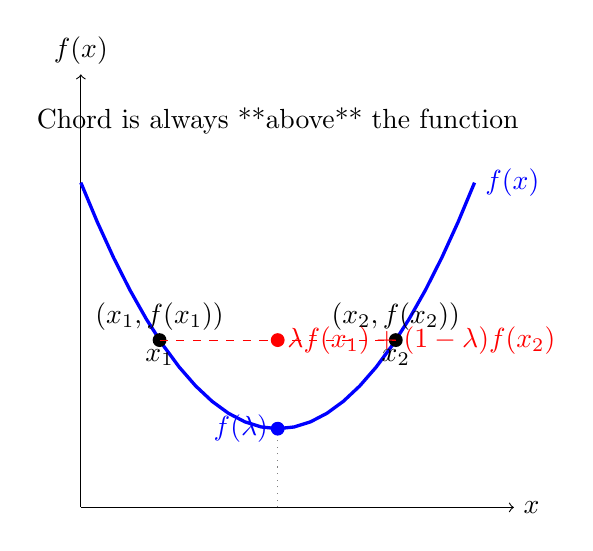
\begin{tikzpicture}[domain=0:5]
    % Define the convex function (e.g., f(x) = 0.5 * (x-2.5)^2 + 1)
    \draw[->] (0,0) -- (5.5,0) node[right] {$x$};
    \draw[->] (0,0) -- (0,5.5) node[above] {$f(x)$};

    % Draw the function f(x)
    \draw[very thick, blue] plot (\x, {0.5 * (\x-2.5)^2 + 1}) node[right] {$f(x)$};

    % Define two points on the x-axis
    \def\xone{1}
    \def\xtwo{4}

    % Calculate the function values
    \pgfmathsetmacro\yone{0.5 * (\xone-2.5)^2 + 1}
    \pgfmathsetmacro\ytwo{0.5 * (\xtwo-2.5)^2 + 1}

    % Draw the points on the graph
    \fill[black] (\xone, \yone) circle (2.5pt) node[below] {$x_1$};
    \fill[black] (\xtwo, \ytwo) circle (2.5pt) node[below] {$x_2$};
    \node at (\xone, \yone + 0.3) {$(x_1, f(x_1))$};
    \node at (\xtwo, \ytwo + 0.3) {$(x_2, f(x_2))$};

    % Draw the chord (line segment) connecting the two points
    \draw[dashed, red] (\xone, \yone) -- (\xtwo, \ytwo);

    % Illustrate a point on the segment and the corresponding function value
    \def\lambdaa{0.5} % Choose lambda = 0.5 for the midpoint
    \pgfmathsetmacro\xlambda{\lambdaa*\xone + (1-\lambdaa)*\xtwo}
    \pgfmathsetmacro\fval{0.5 * (\xlambda-2.5)^2 + 1}
    \pgfmathsetmacro\ycord{\lambdaa*\yone + (1-\lambdaa)*\ytwo}

    % Draw the point on the function
    \draw[dotted, gray] (\xlambda, 0) -- (\xlambda, \fval);
    \fill[blue] (\xlambda, \fval) circle (2.5pt) node[left] {$f(\lambda)$};

    % Draw the point on the chord
    \fill[red] (\xlambda, \ycord) circle (2.5pt) node[right] {$\lambda f(x_1) + (1-\lambda)f(x_2)$};

    % Label the key inequality
    \node[anchor=north] at (2.5, 5.2) {Chord is always **above** the function};

\end{tikzpicture}
\section{Complex Analysis}
\section{Linear Algebra}
\section{Multivariable Calculus}
\section{Useful Tools}
\subsection{Convolution}
\subsubsection{Discrete Series}
\subsubsection{Continuous}
\subsection{Fourier Transform}
\subsection{Laplace Transform}
\subsection{Z Transform}
\section{ODEs}
\section{PDEs}
